%REPORT TEMPLATE
%AUTHOR: RUI QU  
%EMAIL: RQU@KTH.SE 

%----------------------------------------------------------------------------------------
%	PACKAGES AND DOCUMENT CONFIGURATIONS
%----------------------------------------------------------------------------------------

\documentclass{article}

%---Basic---
\usepackage{natbib} % Required to change bibliography style to APA
\usepackage{amsmath} % Required for some math elements 
\setlength\parindent{0pt} % Removes all indentation from paragraphs
\usepackage{listings}%Insert code
\usepackage{times} % Uncomment to use the Times New Roman font

%---Table---
\usepackage{multirow}%Table
\usepackage{booktabs}%Table Triple-lines
\usepackage{siunitx} % Provides the \SI{}{} and \si{} command for typesetting SI units

%---Figure---
\usepackage{graphicx} % Required for the inclusion of images
\usepackage{subfigure} % Required for multiple images
\usepackage{float} 

%---Pseudo-code in LaTeX---
\usepackage{minted} %Preference->engine->pdfTeX->Latex  ADD: -shell-escape
\usepackage{xcolor}
\definecolor{bg}{rgb}{0.95,0.95,0.95}

\usepackage{algorithm}
\usepackage{algpseudocode}
\usepackage{amsmath}
\renewcommand{\algorithmicrequire}{\textbf{Input:}}  % Use Input in the format of Algorithm
\renewcommand{\algorithmicensure}{\textbf{Output:}} % Use Output in the format of Algorithm

%---Appendix---
\usepackage{appendix}
\newcommand{\upcite}[1]{\textsuperscript{\textsuperscript{\cite{#1}}}} %Upcite

%----------------------------------------------------------------------------------------
%	DOCUMENT INFORMATION
%----------------------------------------------------------------------------------------

\begin{document}

\title{CS-E5710 Bayesian Data Analysis\\Assignment 4 }                  
%\author{Rui Qu\\rui.qu@aalto.fi}
\maketitle

% If you wish to include an abstract, uncomment the lines below
% \begin{abstract}
% Abstract text
% \end{abstract}

%----------------------------------------------------------------------------------------
%	SECTION 1
%----------------------------------------------------------------------------------------

\section{Bioassay model and importance sampling}
\textbf{a)} Report the mean and covariance of the bivariate normal distribution
\begin{minted}[bgcolor=bg, linenos, fontsize=\footnotesize]{python}  
mu_a = 0
sigma_a = 2
mu_b = 10
sigma_b = 10
corr = 0.5

mean = np.array([mu_a, mu_b])
print('mean:',mean)

cov = np.array([[sigma_a**2, corr * sigma_a * sigma_b], 
	[corr * sigma_a * sigma_b, sigma_b**2]])
print('covariance:',cov)
\end{minted}

\begin{minted}[bgcolor=bg, linenos, fontsize=\footnotesize]{bash}
mean: [ 0 10]  
covariance: [[  4.  10.]
	 [ 10. 100.]]
\end{minted}
 
 
\textbf{b)} Implement a function for computing the logarithm of the density of the prior distribution
\begin{minted}[bgcolor=bg, linenos, fontsize=\footnotesize]{python}  
def p_log_prior(alpha, beta):

    prior= stats.multivariate_normal(mean, cov)
    pos = np.dstack((alpha, beta))
    log_prior = prior.logpdf(pos)

    return log_prior
    
print('test prior:',p_log_prior(3,9))
\end{minted}

\begin{minted}[bgcolor=bg, linenos, fontsize=\footnotesize]{bash}
test prior: -6.296434970404113
\end{minted}

\textbf{c)} Implement a function for computing the logarithm of the density of the posterior

\begin{equation}
log(posterior)=log(prior\times likelihood)=log(prior)+log(likelihood)
\end{equation}
where $log(likelihood)$ is given in part c), $log(likelihood)$ is given in the BDA repository on GitHub. According to the Chapter3.7 Example: analysis of a bioassay experiment, we could implement $p\_log\_posterior$ as following: 
\begin{minted}[bgcolor=bg, linenos, fontsize=\footnotesize]{python}  
dose = np.array([-0.86, -0.30, -0.05, 0.72])
deaths = np.array([0, 1, 3, 5])
animals = np.array([5, 5, 5, 5])

def p_log_posterior(alpha, beta, x, y, n):
#logarithm of the density of the prior distribution 
    prior= stats.multivariate_normal(mean, cov)
    pos = np.dstack((alpha, beta))
    log_prior = prior.logpdf(pos)
    
#logarithm of the density of the likelihood distribution 
    alpha = np.expand_dims(alpha, axis=-1)
    beta = np.expand_dims(beta, axis=-1)
    t = alpha + beta*x
    et = np.exp(t)
    z = et/(1.+et)
    log_likelihood = np.sum(y*np.log(z)+ (n-y)*np.log(1.0-z), axis=-1)
##logarithm of the density of the posterior distribution 
    log_posterior = log_prior + log_likelihood
    return log_posterior 
    
print('test posterior',p_log_posterior(3, 9, dose, deaths, animals))
\end{minted}

\begin{minted}[bgcolor=bg, linenos, fontsize=\footnotesize]{bash}
test posterior: -15.788012556775058
\end{minted}

\textbf{d)} Plot the posterior density in a grid of points $\alpha\in[-4,4],\ \beta\in[-10,30]$\\


\begin{minted}[bgcolor=bg, linenos, fontsize=\footnotesize]{python}      
alpha, beta = np.meshgrid(np.linspace(-4,4,100),np.linspace(-10,30,100))
posterior = np.exp(p_log_posterior(alpha, beta, dose, deaths, animals))

plt.contourf(alpha, beta,posterior, cmap=plt.cm.Greys)
plt.xlabel('alpha')
plt.ylabel('beta')
plt.title('Posterior Distribution')
plt.grid(linewidth=0.8, alpha=0.2)
plt.colorbar(plt.contourf(alpha, beta, posterior, cmap=plt.cm.Greys))
plt.savefig('./log_posterior.png')
plt.show()
\end{minted}

\begin{figure}[H]
\centering  
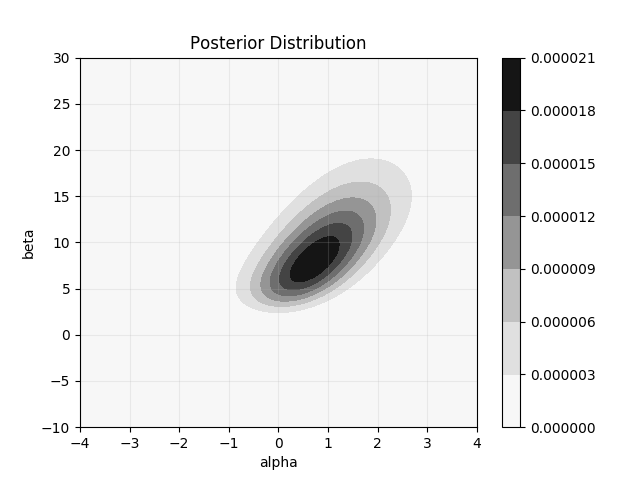
\includegraphics[scale=0.6]{log_posterior.png}
\caption{Heatmap of the posterior density}
\label{fig: label}
\end{figure}
 
\textbf{e)} Sample draws of alpha and beta from the prior distribution
\begin{minted}[bgcolor=bg, linenos, fontsize=\footnotesize]{python}     
prior = stats.multivariate_normal(mean, cov)
samples = prior.rvs(10000)
\end{minted}
Compute the importance ratios (importance weights) for each draw when the target distribution is the posterior distribution.
 
\begin{equation}
\begin{aligned}
&w=\theta_i^{y_i}(1-\theta_i)^{n_i-y_i}\\
&\theta_i=\frac{1}{1+exp(-{\alpha+\beta x_i})}
\end{aligned}
\end{equation}

Normalize the weights so that they sum to 1.
\begin{equation}
\tilde{\mathbf{w}}(\theta^s)=\frac{\mathbf{w}(\theta^s)}{\sum^S_{s'=1}\mathbf{w}(\theta^{s'})}
\end{equation}
\begin{minted}[bgcolor=bg, linenos, fontsize=\footnotesize]{python}     
theta =1/(1+np.exp(-(samples[:,0,None] + samples[:,1,None]*dose)))
weights = np.prod(
    theta**deaths * (1 - theta)**(animals - deaths), axis=1)
    
#Normalize the weights
weights_norm = (weights) / np.sum(weights)
\end{minted}
 
\textbf{f)} Compute the posterior mean using importance sampling and draws from e)

\begin{minted}[bgcolor=bg, linenos, fontsize=\footnotesize]{python}    
posterior_mean = sum(weights[ : , None] * samples) / sum(weights)
print('posterior mean of alpha : ', posterior_mean[0])
print('posterior mean of beta  : ', posterior_mean[1])
 \end{minted}
 
\begin{minted}[bgcolor=bg, linenos, fontsize=\footnotesize]{bash}
posterior mean of alpha: 0.96466253 
posterior mean of beta: 10.48528471
\end{minted}
 
 \textbf{g)} Compute the effective sample size
 
\begin{equation}
\begin{aligned}
&S_{eff}=\frac{1}{\sum^S_{s=1}(\tilde{\mathbf{w}}(\theta^s))^2}\\
&\tilde{\mathbf{w}}(\theta^s)=\frac{\mathbf{w}(\theta^s)}{\sum^S_{s'=1}\mathbf{w}(\theta^{s'})}
\end{aligned}
\end{equation}
\begin{minted}[bgcolor=bg, linenos, fontsize=\footnotesize]{python} 
s_eff = 1 / np.sum(weights_norm**2)
print('effective sample size: ', s_eff)
\end{minted}

\begin{minted}[bgcolor=bg, linenos, fontsize=\footnotesize]{bash}
effective sample size: 2750.282727444427
\end{minted}
 
\textbf{h)} Use importance resampling without replacement to obtain a posterior sample of size 1000 of alpha and beta 

\begin{minted}[bgcolor=bg, linenos, fontsize=\footnotesize]{python}
scode = np.random.choice(a=10000,size=1000,replace=False,p=weights_norm)
resamples = samples[scode]
print('mean of resampled alpha: ', np.mean(resamples[:, 0]))
print('mean of resampled beta: ', np.mean(resamples[:, 1]))
\end{minted}

\begin{minted}[bgcolor=bg, linenos, fontsize=\footnotesize]{bash}
mean of resampled alpha: 0.9247278915535617
mean of resampled beta: 10.650671142369971
\end{minted}

Plot a scatterplot of the obtained posterior sample
\begin{minted}[bgcolor=bg, linenos, fontsize=\footnotesize]{python}
plt.xlim([-4, 4])
plt.ylim([-10, 30])
plt.xlabel('alpha')
plt.ylabel('beta')
plt.grid(linewidth=0.8, alpha=0.2)
plt.scatter(resamples[:, 0], resamples[:, 1],8,color='grey')
plt.title('Posterior Samples')
plt.savefig('./posterior_samples.png')
plt.show()

plt.xlim([-4, 4])
plt.ylim([-10, 30])
plt.xlabel('alpha')
plt.ylabel('beta')
plt.grid(linewidth=0.8, alpha=0.2)
plt.contourf(alpha, beta, posterior, cmap=plt.cm.Greys)
plt.colorbar(plt.contourf(alpha, beta, posterior, cmap=plt.cm.Greys))
plt.scatter(resamples[:, 0], resamples[:, 1], 8, alpha=.15, color='grey')
plt.title('Contourf & Ccatter Comparision')
plt.savefig('./contourf_scatter.png')
plt.show()
\end{minted}
 
\begin{figure}[H]
\centering  
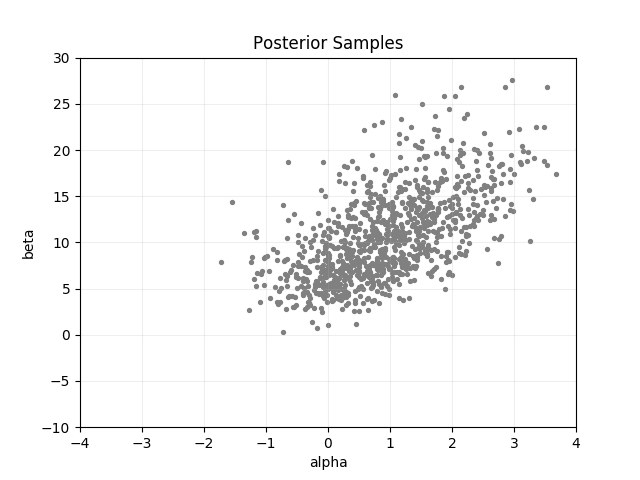
\includegraphics[scale=0.6]{posterior_samples.png}
\caption{Scatterplot of the obtained posterior sample}
\label{fig: label}
\end{figure}

\begin{figure}[H]
\centering  
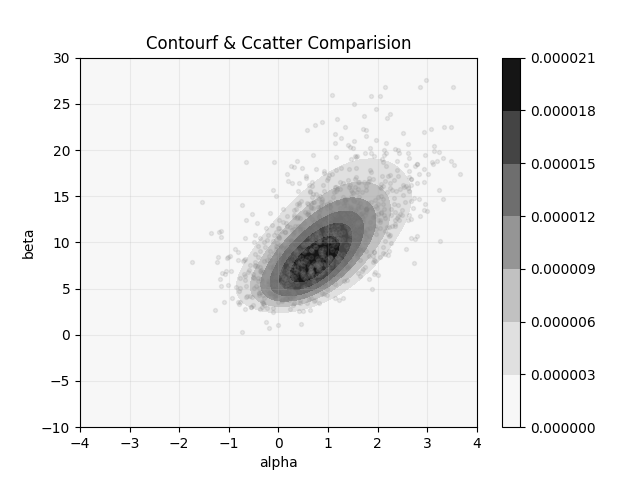
\includegraphics[scale=0.6]{contourf_scatter.png}
\caption{Comparison of Scatterplot and Heatmap }
\label{fig: label}
\end{figure}
 
\textbf{i)} Using the posterior sample obtained via importance resampling, report an estimate for $p(\beta> 0|x, n, y)$, i.e., the probability that the drug is harmful.

\begin{minted}[bgcolor=bg, linenos, fontsize=\footnotesize]{python} 
beta_resample = resamples[:, 1]
alpha_resample = resamples[:, 0]
pos = beta_resample > 0
p_harmful = (beta_resample[pos].size/(beta_resample.size + 1))
print('Probability that the drug is harmful:', p_harmful)
\end{minted}

\begin{minted}[bgcolor=bg, linenos, fontsize=\footnotesize]{bash}  
Probability that the drug is harmful: 0.999000999000999
\end{minted}
 
 
\textbf{j)}  Using the posterior sample obtained via importance resampling, draw a histogram of the draws from the posterior distribution of the LD50 conditional on $\beta>0$\\
 
LD50 is $x_i=-\frac{\alpha}{\beta}$
\begin{minted}[bgcolor=bg, linenos, fontsize=\footnotesize]{python}  
ld50 = - alpha_resample[pos]/beta_resample[pos]
y = np.arange(-0.4, 0.4, 0.01)
plt.hist(ld50, y, ec='white', color='grey')

plt.xlabel('LD50')
plt.title('Histogram')
plt.savefig('./histogram.png')
plt.show()
\end{minted}

\begin{figure}[H]
\centering  
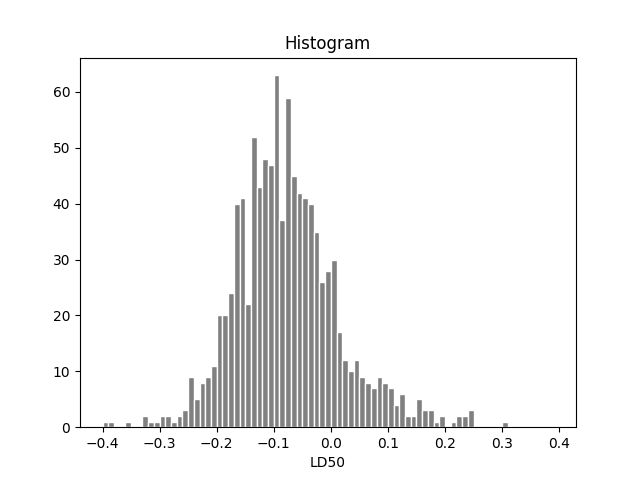
\includegraphics[scale=0.6]{histogram.png}
\caption{Histogram}
\label{fig: label}
\end{figure}

\appendix
\section{Code}
\begin{minted}[bgcolor=bg, linenos, fontsize=\footnotesize]{python} 
import matplotlib.pyplot as plt
from mpl_toolkits.mplot3d import Axes3D
from scipy import stats
import numpy as np

def bioassaylp(a, b, x, y, n):
    # last axis for the data points
    a = np.expand_dims(a, axis=-1)
    b = np.expand_dims(b, axis=-1)
    # these help using chain rule in derivation
    t = a + b*x
    et = np.exp(t)
    z = et/(1.+et)
    # negative log posterior (error function to be minimized)
    lp = np.sum(y*np.log(z)+ (n-y)*np.log(1.0-z), axis=-1)
    return lp
'''
a)
'''
mu_a = 0
sigma_a = 2
mu_b = 10
sigma_b = 10
corr = 0.5

mean = np.array([mu_a, mu_b])
print('mean:',mean)

cov = np.array([[sigma_a**2, corr * sigma_a * sigma_b], 
[corr * sigma_a * sigma_b, sigma_b**2]])
print('covariance:',cov)

alpha,beta = np.meshgrid(np.linspace(-4,4,100), np.linspace(-10,30,100))

'''
b)
'''

def p_log_prior(alpha, beta):

    prior= stats.multivariate_normal(mean, cov)
    pos = np.dstack((alpha, beta))
    log_prior = prior.logpdf(pos)

    return log_prior
#print('test',p_log_prior(3,9))

dose = np.array([-0.86, -0.3, -0.05, 0.72])
deaths = np.array([0, 1, 3, 5])
animals = np.array([5, 5, 5, 5])

'''
c) 
'''

def p_log_posterior(alpha, beta, x, y, n):
    prior= stats.multivariate_normal(mean, cov)
    pos = np.dstack((alpha, beta))
    log_prior = prior.logpdf(pos)

    alpha = np.expand_dims(alpha, axis=-1)
    beta = np.expand_dims(beta, axis=-1)
    t = alpha + beta*x
    et = np.exp(t)
    z = et/(1.+et)
    log_likelihood = np.sum(y*np.log(z)+ (n-y)*np.log(1.0-z), axis=-1)

    log_posterior = log_prior + log_likelihood

    return log_posterior 
#print('testposterior',p_log_posterior(3, 9, dose, deaths, animals))

'''
d) 
'''
alpha,beta = np.meshgrid(np.linspace(-4,4,100), np.linspace(-10,30,100))
posterior = np.exp(p_log_posterior(alpha, beta, dose, deaths, animals))
plt.contourf(alpha, beta,posterior, cmap=plt.cm.Greys)
plt.xlabel('alpha')
plt.ylabel('beta')
plt.title('Posterior Distribution')
plt.grid(linewidth=0.8, alpha=0.2)
plt.colorbar(plt.contourf(alpha, beta, posterior, cmap=plt.cm.Greys))
plt.savefig('./log_posterior.png')
plt.show()

'''
e) 2. Sample draws of alpha and beta from the prior distribution.
'''
prior = stats.multivariate_normal(mean, cov)
samples = prior.rvs(10000)
#print('Shape of the samples from prior: ', samples.shape)

theta = 1 / (1+np.exp(-(samples[:,0,None] + samples[:,1,None] * dose)))
weights = np.prod(
    theta**deaths * (1 - theta)**(animals - deaths), axis=1)

weights_norm = (weights) / np.sum(weights)
#print('Shape of the weights of the likelihood: ', weights.shape)

'''
f) 
'''
posterior_mean = sum(weights[ : , None] * samples) / sum(weights)
print('posterior mean of alpha : ', posterior_mean[0])
print('posterior mean of beta  : ', posterior_mean[1])

'''
g) 
'''
s_eff = 1 / np.sum(weights_norm**2)
print('effective sample size: ', s_eff)

'''
h) 
'''
scode = np.random.choice(a=10000,size=1000,replace=False,p=weights_norm)
resamples = samples[scode]
print('mean of resampled alpha: ', np.mean(resamples[:, 0]))
print('mean of resampled beta: ', np.mean(resamples[:, 1]))

plt.xlim([-4, 4])
plt.ylim([-10, 30])
plt.xlabel('alpha')
plt.ylabel('beta')
plt.grid(linewidth=0.8, alpha=0.2)
plt.scatter(resamples[:, 0], resamples[:, 1],8,color='grey')
plt.title('Posterior Samples')
plt.savefig('./posterior_samples.png')
plt.show()

plt.xlim([-4, 4])
plt.ylim([-10, 30])
plt.xlabel('alpha')
plt.ylabel('beta')
plt.grid(linewidth=0.8, alpha=0.2)
plt.contourf(alpha, beta, posterior, cmap=plt.cm.Greys)
plt.colorbar(plt.contourf(alpha, beta, posterior, cmap=plt.cm.Greys))
plt.scatter(resamples[:, 0], resamples[:, 1], 8, alpha=.15, color='grey')
plt.title('Contourf & Ccatter Comparision')
plt.savefig('./contourf_scatter.png')
plt.show()

'''
i) 
'''
beta_resample = resamples[:, 1]
alpha_resample = resamples[:, 0]
pos = beta_resample > 0
p_harmful = (beta_resample[pos].size/(beta_resample.size + 1))
print('Probability that the drug is harmful:', p_harmful)

'''
j)
'''
ld50 = - alpha_resample[pos]/beta_resample[pos]
y = np.arange(-0.4, 0.4, 0.01)
plt.hist(ld50, y, ec='white', color='grey')
plt.xlabel('LD50')
plt.title('Histogram')
plt.savefig('./histogram.png')
plt.show()

\end{minted}

\end{document}